\chapter*{Preface}

\begin{comment}
  Throughout history, scientific fields have split, merged and been made obsolete. What we find important is dictated by our philosophical ideals, economic status, cultural norms and scientific curiosity. The current frontiers of science aim probe our understandings of the very laws of physics through our studies of the exotic Higgs boson to recreating the wistful alchemical dream of artificial atoms through quantum dots. Corporeally, we have staked out the biological form as new fertile ground for us explore and pioneer. The explosive growth in this interest, fueled by new technologies, has lead to the growth of a new multi-disciplined approach called biophysics.
\end{comment}

Traditionally, the components of biophysics, biology and physics, have a tangential mode of thought.  Biology, the study of living things, is a field governed by qualitative observation and later mathematical models are applied. Prediction comes from the understanding of the various mechanisms that are often intricately coupled. On the other hand, a mature branch of physics is governed by the mathematical form first. Ideas are founded from first principles, from which the physical laws are then derived. If these predictions fail to accurately portray reality the fundamental assumptions are discarded and presumed to be false. The successful theories in physics have a far greater precision than the biological counterparts. How then do the two fields reconcile, the dogma of each being so different?
%
\begin{equation*}
  \chem{bioPHYSICS \longleftrightarrow BIOphysics}
\end{equation*}

In this author’s opinion, the field of biophysics has truly made possible by a third kind of science. After experiment and theory comes modeling, an approach that has been greatly enhanced by the use of modern day computers. Scientific modeling incorporates rigorous mathematical derivations, yet the results are interpreted as though they were experimental evidence. It is rapidly being recognized as an important and vital component to our scientific endeavors.\cite{reed_computational_2005} In some ways modeling takes the best of both forms, allowing each to contribute. This approach has been used in many diverse fields such as meteorology, economics, and our present topic, biophysics.

Biophysics has an implicit scale. Usually the scale spans from collections of cells (on order of microns) to collections of atoms (on order of angstroms). As an example of the types of objects currently studied, Figure \ref{fig:conf_words} shows the usage of the words found in abstracts of presentations and posters at a recent biophysics conference. The three dominant objects that were studied were proteins, cells, and membranes. The larger structures (except in the cases of aggregation) traditionally studied in biology are out of the scope of most biophysical studies. 
%
\begin{figure}
  \begin{centering}
    \fbox{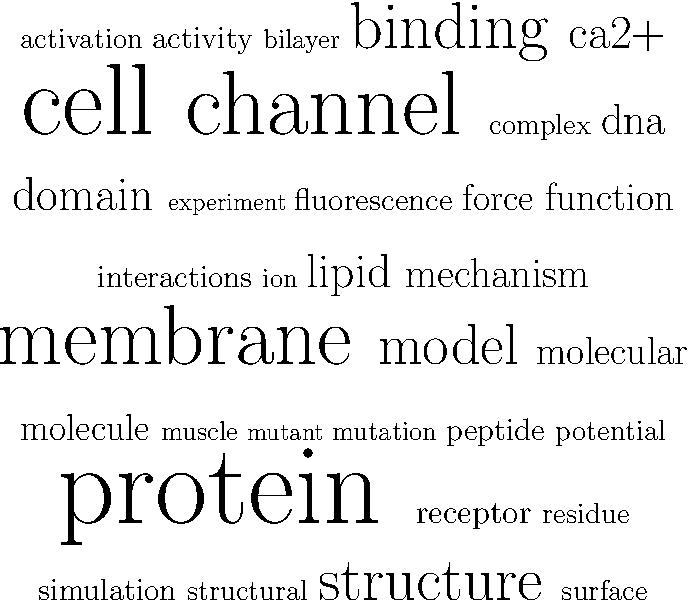
\includegraphics[height=5 cm]
      {pictures/wordcloud_conf/abstract_wordcloud.pdf}}
    \caption{Snapshot of the most commonly used words in the abstracts of the 2010 Biophysical Conference in San Francisco.\cite{BPS_conf_2010} Larger words correspond to a greater usage. Note that the prominent words, protein, cell, and membrane set the length scale that narrows the focus of the discipline.}
    \label{fig:conf_words}
  \end{centering}
\end{figure}

As we move to smaller structures we find ourselves in the realm of quantum chemistry and pure physics. In this regime, theories of ``first-principle'' abound. That is, starting from a set of empirically verified postulates, equations are derived which predict the dynamics and structure of the system. As we move to larger structures we are back in the traditional biological realm, where the role of classification dictates the functionality. 
For the theoretical and modeling based biophysicist the aim is to derive from first-principle equations. The attempt is to classify and organize the higher-order structures found at this scale. The predictions must ultimately be vetted by experiment studies, thus neither group can work in isolation.
%The approach of a biophysicist, due to its multi-disciplined nature, often depends on the formal training of the scientist conducting the experiment. Pure observationalists and theorists exist, often coming from their respective fields, but their appearance is the exception rather than the rule. Sampling from the abstracts of a recent meeting of the Biophysical Societies 2010 Annual Meeting \cite{BPS_conf_2010}, the largest in it's field with a few thousand talks, symposia and poster presentation, one finds that many scientists are engaged in the modeling approach, from the development to the interpretation. 

It is here that we begin our discussion, at the crossroads of two diverse fields whose singular aim is no less than the understanding of the phenomena behind life itself.

